\subsection{DSOA - \emph{Device Service Oriented Architecture}}

A DSOA foi definida baseada na arquitetura SOA(\emph{Service Oriented Architecture}) que possui diversas características que podem auxiliar ambientes inteligentes como a capacidade da reutilização de recursos de software. Entretanto, por ser uma apenas uma arquitetura genérica, não leva em consideração características e limitações de ambientes inteligentes, descrevendo apenas serviços em alto nível e não define, ainda, um modelo de comunicação.

Na DSOA destacam-se cinco conceitos básicos:

\begin{itemize}
	\item Ambiente Inteligente:

		É um ambiente composto por pelo menos dois dispositivos capacidade de computação e conectados por meio de uma rede de comunicação coloborativa com os usuários do ambiente. O provimento de serviços para o usuário vem da interação das aplicações deste ambiente dinâmico. Essa dinamicidade do ambiente ubíquo se dá pelo fato que os usuários entram, saem e se movimentam no ambiente, além disso, trazem consigo seus dispositivos. É importante ressaltar que um ambiente inteligente neste trabalho não tem seu significado mais popular de ambiente com inteligência artificial.
	\item Dispositivo:

		É um aparelho que possua capacidade de comunicação e que abrigar aplicações ou disponibilizar seus recursos do ambiente inteligente para que outras aplicações possam utilizar de seus serviços.
	\item Recurso:

		É um grupo de funcionalidades relacionadas que podem ser acessadas por meio de interfaces pré-definidas.
		\begin{itemize}
			\item Interface do Recurso:

				O recurso é a entidade básica de interação entre dispositivos, visto que é por meio dele que as funcionalidades presentes no ambiente poderão ser acessadas. Para que isso possa é acontecer, é necessário que seja definida uma interface de comunicação que seja conhecida pelas entidades presentes no \emph{smart space}. Essa interface é constituída por dois elementos:
				\begin{itemize}
					\item Identificador:

						Responsável por identificar unicamente um recurso entre diversos recursos presentes no ambiente.
					\item Conjunto de serviços:

						Conjunto de serviços que constituem o recurso e são disponibilizados por ele.
				\end{itemize}
		\end{itemize}
	\item Serviço:

		É a implementação de uma funcionalidade disponibilizada para o ambiente pelo reucurso e uma interface conhecida.
		\begin{itemize}
			\item Interface do Serviço:
			\begin{itemize}
				\item Recurso:

					Recurso do qual o serviço faz parte. Os serviços são encontrados a partir dos recursos.
				\item Identificador:

					Responsável por identificar unicamente um serviço dentro do recurso.
				\item Parâmetros:

					Parâmetros que serão passados para o serviços realizar a funcionalidade requisitada.
			\end{itemize}
		\end{itemize}
	\item Aplicações:
	
		São as responsáveis pela implementação da inteligência do ambiente. As aplicações executam nos dispositivos presentes no ambiente e, a partir de informações providas pelos recursos do amibente, podem realizar ações. Elas interagem com o usuário intermediando suas ações junto ao ambiente. Elas funcionam se relacionando com recursos para notificar o usuário da alteração de algum estado, ou aguardam a execução de algum comando por parte do usuário.
\end{itemize}

\begin{figure}[ht]
	\center
	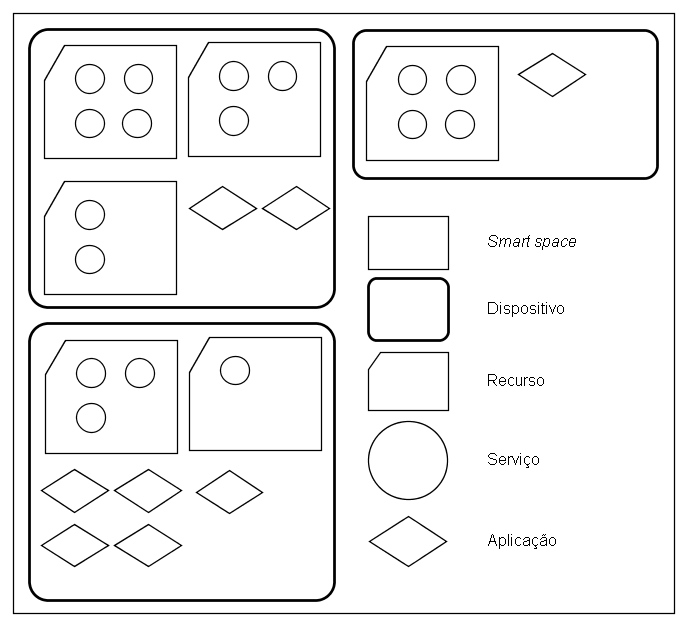
\includegraphics[scale=0.6]{imagens/arquiteturaDSOA}
	\caption{Exemplo da arquitetura DSOA.}
	\label{fig:arquiteturaDSOA}
\end{figure}